\PassOptionsToPackage{svgnames}{xcolor}
\documentclass[12pt]{article}



\usepackage[margin=1in]{geometry}  
\usepackage{algorithm,algpseudocode}
\newcommand{\vars}{\texttt}
\newcommand{\func}{\textrm}
\usepackage{graphicx}             
\usepackage{amsmath}              
\usepackage{amsfonts}
\usepackage{framed}               
\usepackage{amssymb}
\usepackage{array}
\usepackage{amsthm}
\usepackage{multirow}
\usepackage[nottoc]{tocbibind}
\usepackage{bm}
\usepackage{enumitem}
\usepackage{tikz}
\usepackage{pdfpages}
\usepackage{tabularx}
\algdef{SE}[SUBALG]{Indent}{EndIndent}{}{\algorithmicend\ }%
\algtext*{Indent}
\algtext*{EndIndent}
\newcolumntype{C}[1]{>{\centering\let\newline\\\arraybackslash\hspace{0pt}}m{#1}}
\newcommand\norm[1]{\left\lVert#1\right\rVert}
\setlength{\parindent}{0cm}
\setlength{\parskip}{0em}
\newcommand{\ind}{\hspace*{15pt}}
\newcommand{\Lim}[1]{\raisebox{0.5ex}{\scalebox{0.8}{$\displaystyle \lim_{#1}\;$}}}
\newtheorem{definition}{Definition}[section]
\newtheorem{theorem}{Theorem}[section]
\newtheorem{notation}{Notation}[section]
\theoremstyle{definition}
\DeclareMathOperator{\arcsec}{arcsec}
\DeclareMathOperator{\arccot}{arccot}
\DeclareMathOperator{\arccsc}{arccsc}
\DeclareMathOperator{\spn}{Span}
\DeclareMathOperator{\diff}{d}
\setcounter{tocdepth}{1}
\begin{document}
\title{Revision notes - CS3244}
\author{Ma Hongqiang}
\maketitle
\tableofcontents

\clearpage
%\twocolumnt
\section{Introduction}
\begin{definition}[Learning]
\hfill\\\normalfont
An agent is said to be \textbf{learning} if it improves its performance $P$ on task $T$ based on experience $E$.\\
Here $T$ must be fixed, $P$ be measurable and $E$ must exist.
\end{definition}
It is useful for the agent to learn since it could be hard to preprogram the agent's strategy, hard to encode all human knowledge, and less to program.
\begin{definition}[Design of Learning Agent]
\hfill\\\normalfont \begin{figure}[h]
\centering
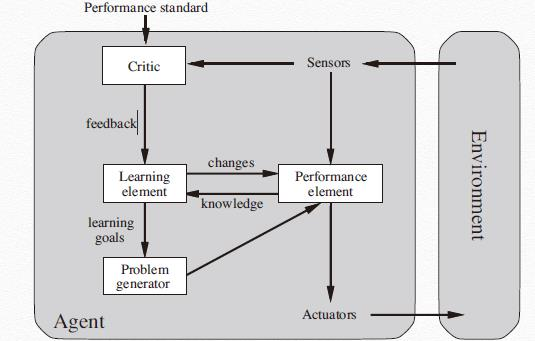
\includegraphics[width=0.7\textwidth]{1-1.jpg}
\end{figure}
Here, the performance element selects the external actions and sends to actuators.\\
The learning element takes in critic's output and improves agent to perform better, by updating the performance element.\\
The critic gives feedback on how well the agent is doing.\\
The problem generator suggests explorative actions that will lead to new, informative, but not necessarily better experience.
\end{definition}
The design of the learning agent is affected by
\begin{itemize}
	\item Which components of the performance element are to be learned
	\item What representation is used for data and the components
	\item What feedback is available to learn these components
\end{itemize}
The types of feedback include:
\begin{itemize}
	\item \textbf{Supervised learning}: correct answer given for each example
	\item \textbf{Unsupervised learning}: correct answers not given
	\item \textbf{Reinforcement learning}: occasional rewards given
\end{itemize}
\clearpage

\section{Concept Learning}
\begin{definition}[Concept, concept learning]
\hfill\\\normalfont A concept is a boolean-valued function over a set of input instances, each comprising input attributes.\\
\textbf{Concept learning} is a form of \textbf{supervised learning}. It is to infer an unknown \textbf{boolean valued function} from \textit{training examples}.
\end{definition}
\begin{definition}[Hypothesis]
\hfill\\\normalfont \textbf{Hypothesis} $h$ is a conjunction of constraints on input attributes, where each \textbf{constraint} can be:
\begin{itemize}
	\item A specific value, e.g. \texttt{water = warm}
	\item Don't care, e.g. \texttt{water = ?}
	\item No value allowed, e.g. \texttt{water = }$\varnothing$
\end{itemize}
\end{definition}
Since conjunction is commutative, we can represent a hypothesis in an unordered list like
\begin{table}[h]
\centering
\begin{tabular}{|c|c|c|c|}
\hline
Sky & AirTemp & Humidity & Wind\\\hline
Sunny & ? & ? & Strong \\\hline
\end{tabular}
\end{table}
To learn using concept learning, we are given input instances $X$. Each instance $x\in X$ is represented by the a list of input attributes describing the state, in the form of \texttt{key, value}, where \texttt{value} is an element from teh set of values corresponding to the \texttt{key}.\\
We are also given hypothesis space $H$. Each hypothesis $h\in H$ with the form $h: X\to \{0,1\}$ is represented by a conjunction of constraints on input attributes.
\begin{definition}[Satisfying Hypothesis]
\hfill\\\normalfont An input instance $x\in X$ \textbf{satisfies} all constraints of a hypothesis $h\in H$ iff $h(x)=1$.
\end{definition}
In other words, $h$ classifies $x$ as a positive example.\\
\begin{definition}[Aim of Training]
\hfill\\\normalfont Given unknown \textbf{target concept} $c: X\to \{0,1\}$, and \textit{noise-free} training examples $D =  \{\langle x_1, c(x_1)\rangle, \ldots, \langle x_n, c(x_n)\rangle\}$, determine a hypothesis $h\in H$ that is \textbf{consistent} with $D$.\\
Here, a hypothesis is \textbf{consistent} with training example $D$ \textit{if and only if} $h(x)=c(x)$ for all $\langle x, c(x)\rangle\in D$.
\end{definition}
Here, we have this \textbf{inductive learning assumption}: any hypothesis found to approximate the target function well over a \textit{sufficiently large set of training examples} will also approximate the target function well over other \textit{unobserved examples}.\\
One can view concept learning as search for a hypothesis $h\in H$ consistent with $D$.\\
Every hypothesis containing 1 or more $\varnothing$ symbols represents an \textbf{empty set} of input instances, hence classifying every instance as a negative example.\\
Usually the hypothesis space $H$ is quite large or even infinite, so we need to exploit structure for searching efficiently.\\
Before we can do this, we defines a relation $\geq_g: H\times H\to \{0,1\}$.
\begin{definition}[More General than or Equal To]
\hfill\\\normalfont $h_j$ is \textbf{more general than or equal to} $h_k$, denoted by $h_j\geq_g h_k$ if and only if any input instance $x$ that satisfies $h_k$ also satisfies $h_j$:
\[
\forall x\in X, h_k(x)=1\Rightarrow h_j(x)=1
\]
\end{definition}
$\geq_g$ relation defines a \textit{partial order} over $H$ and not total order.
\begin{definition}[More General than]
\hfill\\\normalfont $h_j$ is \textbf{more general than} $h_k$, i.e. $h_j>_g h_k$ if and only if $h_j\geq_g h_k$ and $h_k\not\geq_g h_j$.\\
$h_j$ is \textbf{more specific than} $h_k$ if and only if $h_k$ is more general than $h_j$.
\end{definition}
\begin{theorem}[Find-S algorithm]
\hfill\\\normalfont
\begin{itemize}
	\item Initialize $h$ to most specific hypothesis in $H$
	\item For each positive training instance $x$
	\begin{itemize}
		\item For each attribute constraint $a_i$ in $h$,
			\begin{itemize}
				\item if $x$ satisfies constraint $a_i$ in $h$, do nothing
				\item else, replace $a_i$ in $h$ by the next more general constraint that is satisfied by $x$
			\end{itemize}
	\end{itemize}
	\item Output hypothesis $h$
\end{itemize}
\end{theorem}
Essentially, we just run the current most specific hypothesis possible against the remaining training data. After one iteration, we can obtain the hypothesis we want for Find-S algorithm.
\begin{theorem}
\hfill\\\normalfont $h$ is consistent with $D$ if and only if every positive training instance satisfies $h$ and every negative training instance does not satisfy $h$.
\end{theorem}
\begin{theorem}
\hfill\\\normalfont Suppose that $c\in H$. Then $h_n$ is consistent with $D=\{\langle x_k, c(x_k)\rangle\}_{k=1,\ldots, n}$.
\end{theorem}
However, although find-S guarantees to find consistent hypothsis if it exists in hypothesis space, it has the following limitations:
\begin{itemize}
	\item It cannot tell whether find-WS has learned target concept
	\item It cannot tell when training examples are inconsistent
	\item It picks a maximally specific $h$
	\item Depending on $H$, there might be several
\end{itemize}
\begin{definition}[Version Space]
\hfill\\\normalfont The \textbf{version space} $VS_{H,D}$ with respect to hypothesis space $H$ and training examples $D$, is the subset of hypothesis from $H$ that are consistent with $D$:
\[
VS_{H,D}=\{h\in H \mid h \text{ is consistent with } D\}
\]
If $c\in H$, then a large enough $D$ can reduce $VS_{H,D}$ to $\{c\}$. However, if $D$ is sufficient, then the cardinality of $VS_{H,D}$ will be more than 1, which measn that $VS_{H,D}$ represents the \textbf{uncertainty} of what the target concept is.\\
$VS_{H,D}$ contains all consistent hypothesis, which includes the maximally specific hypothesis.
\end{definition}
\begin{theorem}[List-Then-Eliminate Algorithm]
\hfill\\\normalfont \begin{itemize}
\item \textit{VersionSpace}$\leftarrow$ a list containing every hypothesis in $H$
\item For each training example $\langle x, c(x)\rangle$
\begin{itemize}
	\item Remove from \textit{VersionSpace} any hypothesis $h$ for which $h(x)\neq c(x)$.
\end{itemize}
\item Output the list of hypothesis in \textit{VersionSpace}
\end{itemize}
\end{theorem}
This generates the $VS_{H,D}$. However, it is prohibitively exprensive to exhaustively enumerate all hypothesis in finite $H$.
\begin{definition}[General Boundary, Specific Boundary]
\hfill\\\normalfont The \textbf{general boundary} $G$ of $VS_{H,D}$ is the set of \textbf{maximaly general members} of $H$ consistent with $D$:
\[
G=\{g\in H\mid g\text{ consistent with } D \land (\neg \exists g' in H,\text{ s.t. } g'>_g g \land g' \text{ consistent with } D\}
\]
The \textbf{specific boundary} $S$ of $VS_{H,D}$ is the set of maximally specific members of $H$ consistent with $D$.
\[
S=\{s\in H\mid s\text{ consistent with } D \land (\neg \exists s' in H,\text{ s.t. } s>_g s' \land s' \text{ consistent with } D\}
\]
\end{definition}
From the definition, we can see that every member of version space lies \textit{between} these boundaries:
\begin{theorem}[Version Space Representation Theorem]
\hfill\\\normalfont 
\[
VS_{H,D}=\{h\in H\mid \exists s\in S, \exists g\in G g\geq_g h\geq_g s\}
\]
\end{theorem}
\begin{theorem}[Candidate Elimination Algorithm]
\hfill\\\normalfont \begin{itemize}
\item $G\leftarrow$maximally general hypothesis in $H$
\item $S\leftarrow$maximally specific hypothesis in $H$
\item For each training sample $d$
\begin{itemize}
	\item If $d$ is a positive example
	\begin{itemize}
		\item Remove from $G$ any hypothesis inconsistent with $d$
		\item For each $s\in S$ not consistent with $d$
		\begin{itemize}
			\item Remove $s$ from $S$
			\item Add to $S$ all minimal generalizations $h$ of $s$ such that $h$ is consistent with $d$, \textit{and} some member of $G$ is more general than $h$
			\item Remove from $S$ any hypothesis that is more general than another hypothesis in $S$
		\end{itemize}
	\end{itemize}
	\item If $d$ is a negative example
	\begin{itemize}
		\item Remove from $S$ any hypothesis inconsistent with $d$
		\item For each $g\in G$ not consistent with $d$
		\begin{itemize}
			\item Remove $g$ from $G$
			\item Add to $G$ all minimal specifications $h$ of $g$ such that $h$ is consistent with $d$, \textit{and} some member of $S$ is more specific than $h$
			\item Remove from $G$ any hypothesis that is more specific than another hypothesis in $G$
		\end{itemize}
	\end{itemize}	
\end{itemize}
\end{itemize}
\end{theorem}
The candidate elimination algorithm has the following properties:
\begin{itemize}
	\item Error in training data will remove hypothesis inconsistent with the erroneous example, which include target concept $c$\\$S$ and $G$ will reduce to $\varnothing$ with sufficiently large data
	\item Insufficiently expressive hypothesis representation, for example a biased hypothesis space which does not contain $c$, will cause $S$ and $G$ to be reduced to $\varnothing$ with sufficiently large data.
\end{itemize}
To make this algorithm efficient, an active learner should query input instance that satisfies \textit{exactly half} of hypotheses in version space, which reduces the version space by half with each training example.\\
This implies we need at least $\lceil log_2(|VS_{H,D}|)\rceil$ examples to find target concept $c$.
\begin{theorem}\hfill\\\normalfont An input instance $x$ satisfies every hypothesis in $VS_{H,D}$ if and only if $x$ satisfies every member of $S$.
\end{theorem}
The above result is a direct implication from definition of specific boundary $S$.\\
We have a counterpart theorem regarding general boundary $G$:
\begin{theorem}\hfill\\\normalfont An input instance $x$ satisfies none of the hypothesis in $VS_{H,D}$ if and only if $x$ satisfies none of the members of $G$.
\end{theorem}
So we can use these theorems to completely classify new unobserved input instance.\\
Usually when training, an unbiased learner will have a hypothesis space $H$ that can express every teachable concept, which is the power set of $X$. In such setting, we need training examples for every input instance in $X$ to converge to that target concept. The \textbf{limitation} is that it cannot classify new unobserved input isntances.\\
To overcome such limitations, we introduce \textbf{inductive bias}.
\begin{definition}[Inductive Bias]
\hfill\\\normalfont
Given
\begin{itemize}
\item Concept learning algorithm $L$
\item Input isntances $X$, unknown target concept $c$
\item Noise free training examples $D_c=\{\langle x_k\in X, c(x_k)\in \{0,1\}\}_{k=1,\ldots, n}$
\end{itemize}
We use $L(x, D_c)\to \{0,1\}$ to denote the classification of input instance $x$ by $L$ after learning from training example $D_c$.\\
The \textbf{inductive bias} of $L$ is any minimal set of assertions $B$ such that for any target concept $c$ and corresponding training examples $D_c$,
\[
\forall x\in X, (B\land D_c\land x)\models (c(x)=L(x,D_c))
\]
\end{definition}
\begin{theorem}[Inductive Bias of Candidate Elimination]
\hfill\\\normalfont The Inductive bias of candidate elimination is the piece of infomration: $B=\{c\in H\}$.\\
Here, we assume candidate elimination outputs a classification $L(x, D_c)$ of input instance $x$ if this vote among hypothesis in $VS_{H, D_c}$ is unanimously positive or negative, and do not output otherwise.
\end{theorem}
Here, we have three types of learner:
\begin{itemize}
	\item \textbf{Rote-learner}: Store examples and classify input instance $x$ if and only if it matches that of previously observed example. There is \textit{no} inductive bias, since we do not make any induction.
	\item \textbf{Candidate-Elimination}: Inductive bias: $c\in H$.
	\item \textbf{Find-S}: Inductive bias is $c\in H$ and all instance are negative unless the opposite is entailed by its other knowledge.\\
	This is because it only has a specific boundary without any general boundary to begin with.
\end{itemize}、
\clearpage
\section{Decision Tree Learning}
The advantage of decision tree(DT) learning over concept learning is listed in the table below:
\begin{table}[]
\begin{tabular}{|l|l|l|}
\hline
                        & Concept Learning                                                                            & DT Learning                                                                                                                             \\ \hline
Target function/concept & Binary outputs                                                                              & Discrete Outputs                                                                                                                        \\ \hline
Training Data           & Noise-free                                                                                  & Robust to noise                                                                                                                         \\ \hline
Hypothesis space        & Restricted(hard bias)                                                                       & Complete, expressive                                                                                                                    \\ \hline
Search strategy         & \begin{tabular}[c]{@{}l@{}}Complete: version space\\ Refine search per example\end{tabular} & \begin{tabular}[c]{@{}l@{}}Incomplete: prefer shorter tree(soft bias)\\ Refine search using all examples\\ No backtracking\end{tabular} \\ \hline
Exploit structure       & General to specific ordering                                                                & Simple to complex ordering                                                                                                              \\ \hline
\end{tabular}
\end{table}
For decision tree learning, the input instance $X_i=A_1\times \cdots\times A_n$ is described by input attribute values, which can be \texttt{boolean}, discrete or continuous. The classification is still \texttt{positive} or \texttt{negative}.\\
We can think of decision tree as a nother possible representation of hypothesis.\\
Decision tree has the expressive power, which can express any function of input attributes, i.e., $f: A_1\times\cdots\times A_n\to \{0,1\}$. Here, we put the realisation of $A_p$ on the edges, which leads to another attribute $A_q$ or the classification.\\
We would most likely want to find \textbf{compact} decision trees.\\
Note, a \texttt{boolean} decision tree can be expressed in disjunctive normal form. For example, $f(A,B):=A \texttt{XOR} B$ can be expressed as $f(A,B)=(\neg A\land B)\lor (A\land \neq B)$.\\
The more important idea is that we can view each conjunction as a \textbf{path}! The above statement suggests
\[
\text{Goal} \Leftrightarrow (\text{Path}_1\lor\cdots\lor \text{Path}_n)
\]
where each path is a \textbf{conjunction} of attribute-value tests, of the form $\text{test}_1\land \cdots\land \text{test}_m$.\\
The search space for decision tree grows hyper-exponentially. Specifically, the number of distinct binary decision trees with $m$ \texttt{boolean} attributes = $2^{2^m}$, as we have $|\prod_{i=1}^m X_i|=2^m$, and the distinct decision trees is the power set of this set, as each value can go either $0$ or $1$.\\
\subsection{Decision Tree Learning Algorithm}
The aim of decision tree learning is to find a \textbf{small} tree \textbf{consistent} with training examples.\\
We need to \textit{greedily}(which may not be optimal) choose the most ``important'' attribute as root of subtree, which essentially removes duplication in the rest of the tree.\\
\begin{theorem}[Decision Tree Learning Algorithm]
\hfill\\\normalfont
\textbf{function} \textsc{Decision-Tree-Learning}(\textit{examples, attributes, parent\_examples}) \textbf{returns} tree\\
\ind \textbf{if} \textit{examples} is empty \textbf{then return} \textsc{Plurality-Value}(\textit{parent\_examples})\\
\ind \textbf{else if} all \textit{examples} have the same classification \textbf{then return} the classification\\
\ind \textbf{else if} \textit{attributes} is empty \textbf{then return} \textsc{Plurality-Value}(\textit{examples})\\
\ind \textbf{else}\\
\ind\ind $A\leftarrow \arg\max_{a\in \textit{attributes}}$ \textsc{Importance}($a$, \textit{examples})\\
\ind\ind $\textit{tree}\leftarrow$ a new decision tree with root test $A$\\
\ind\ind \textbf{for each} value $v_k$ of $A$ \textbf{do}\\
\ind\ind\ind \textit{exs}$\leftarrow\{e: e\in \textit{examples} \textbf{ and }e.A=v_k \}$\\
\ind\ind\ind \textit{subtree}$\leftarrow\textsc{Decision-Tree-Learning}(\textit{exs}, \textit{attributes}\setminus A, \textit{examples})$\\
\ind\ind\ind add a branch to \texttt{tree} with label $(A=v_k)$ and subtree \textit{subtree}.
\ind\ind \textbf{return} \textit{tree}\\
\end{theorem}
Here, the function \textsc{Plurality-Value} selects the most common output value among a set of examples, breaking ties randomly.\\
The function \textsc{Importance} is related to the notion of information gain, which is defined in terms of \textbf{entropy}, which measures \textbf{uncertainty of classification}.
\begin{definition}[Entropy]
\hfill\\\normalfont Entropy measures uncertainty of random variable $C\in\{c_1,\ldots, c_k\}$:
\[
H(C)=-\sum_{i=1}^k P(c_i)\log_2 P(c_i)
\]
\end{definition}
We can define $B(q)$ as entropy of Boolean variable with probability $q$ to be \texttt{true}, i.e.,
\[
B(q)=-q\log_2 q-(1-q)\log_2(1-q)
\]
For a training set containing $p$ positive examples and $n$ negative examples, entropy of target concept $C$ on this set is
\[
H(C)=B(\frac{p}{p+n})=-\frac{p}{p+n}\log_2\frac{p}{p+n}-\frac{n}{p+n}\log_2\frac{n}{p+n}
\]
Here, some important special case of entropy are:
\begin{itemize}
	\item If $p=n(\neq 0)$, then $H(C)=1$ attains its \textbf{maximum}.
	\item If $p=0$ or $n=0$, then $H(C)=0$, which suggests no uncertainty.
	\item Any other non-zero combinations will attain an entropy in $(0,1)$.
\end{itemize}
Specifically, we note the 2-class entropy $B(\frac{p}{p+n})$ to increase monotonically between $(0,\frac{1}{2})$ and monotonically decreasing between $(\frac{1}{2},1)$.\\
Suppose a chosen attribute $A$ divides the training set $E$ into subset $E_1,\ldots, E_d$ corresponding to the $d$ distinct values of $A$. Each subset $E_i$ has $p_i$ positive and $n_i$ negative examples. Then the expected entropy remaining after testing attribute $A$ is 
\[
H(C\mid A):=\sum_{i=1}^d\frac{p_i+n_i}{p+n}B(\frac{p_i}{p_i+n_i})
\]
\begin{definition}[Information Gain]
\hfill\\\normalfont \textbf{Information Gain} of target concept $C$ from the attribute test on $A$ is the expected reduction in entropy:
\[
\mathrm{Gain}(C,A)=B(\frac{p}{p+n})-H(C\mid A)
\]
where the first term on the RHS is the entropy $H(C)$.
\end{definition}
In the decision tree learning, we choose the attribute $A$ with the largest $\mathrm{Gain}$. This gives the implementation of \textsc{Importance}.\\
In other words, \textsc{Decision-Tree-Learning} uses information gain \textit{heuristic} to search through the space of decision trees, from simplest to increasingly complex.
\begin{theorem}[Inductive Bias of DT Learning]
\hfill\\\normalfont There are 2 inductive bias:
\begin{enumerate}
	\item \textbf{Shorter trees} are preferred.
	\item Trees that place \textbf{high information gain attributes close to the root} are preferred.
\end{enumerate}
\end{theorem}
If we only include $(a)$ in the bias, it is the \textbf{exact} inductive bias of BFS for shortest consistent DT, which is prohibitively expensive.\\
Do note, bias is a \textit{preference} for some hypothesis over the others. Bias does not restrict hypothesis space.
\subsection{Overfitting}
\begin{definition}[Overfit]
\hfill\\\normalfont Hypothesis $h\in H$ \textbf{overfits} the set $D$ of training examples if and only if
\[
\exists h'\in H\setminus\{h\} (\mathrm{error}_D(h)<\mathrm{error}_D(h') \land \mathrm{error}_{D_X}(h)>\mathrm{error}_{D_X}(h'))
\]
where $\mathrm{error}_D(h)$ denotes error of $h$ over $D$; $\mathrm{error}_{D_X}(h)$ denotes erros of $h$ over $D_X$, exmamples corresponding to instance space $X$.
\end{definition}
Here, it is clear that training set $D$ is a subset of instance space $X$.\\
Overfitting is more likely as hypothesis and number of input attribute grows, and less likely if we increase number of training examples.\\
We can avoid overfitting by
\begin{itemize}
	\item Stop growing DT when expanding a node is not \textit{statistically} significant.
	\item Allow DT to grow and overfit the data, and \textbf{then post-prune} it.
\end{itemize}
In order to have a metric measuring the quality of DT, we can measure against
\begin{itemize}
	\item Training data
	\item or a separate \textbf{validation} dataset
	\item Minimum description length, which minimizes the size of tree and size of misclassifications of the tree
\end{itemize}
\begin{theorem}[Reduced-error Pruning]
\hfill\\\normalfont
We here explore ideas of partition data into \textit{training} and \textit{validation} sets. The algorithm is below:\\
Do, until further pruning is harmful:
\begin{enumerate}
	\item Evaluate impact on \textit{validation} set of pruning each possible node (i.e., removing subtree rooted at it)
	\item Greedily remove the one that \textbf{most} improves validation set accuracy
\end{enumerate}
Then, produce the smallest version of the most accurate subtree.
\end{theorem}
\begin{theorem}[Rule Post-Pruning]
\hfill\\\normalfont Convert learned DT to an equivalent set of rules by creating one rule for each path from root to a leaf:
\begin{verbatim}
IF   Rules(conjunction)
THEN Classification
\end{verbatim}
Then prune each rule by removing any precondition that improves its estimated accuracy.\\
Sort pruned rules by estimated accuracy into desired sequence for use, when classifying unobserved input instances.
\end{theorem}
\subsection{Dealing with Attributes}
For continuous-valued attributes, we consider only the discrete set of intervals derived from the continuous values.\\
There is one problem with the guiding function for \textsc{Importance}, the Gain function. In training, Gain will select attribute with \textbf{many values}.\\
To resolve the problem, we define another function called \texttt{GainRatio}:
\begin{definition}[Gain Ratio]
\hfill\\\normalfont 
\[
\texttt{GainRatio}(C,A)= \frac{\mathrm{Gain}(C,A)}{\mathrm{SplitInformation}(C,A)}
\]
where $\mathrm{SplitInformation}(C,A)=-\sum_{i=1}^d\frac{|E_i|}{|E|}\log_2\frac{|E_i|}{|E|}$.
\end{definition}
Another problem arises we want to learn consistent DT with low expected cost. In such case we can replace Gain by things like
\[
\frac{\mathrm{Gain}^2(C,A)}{\mathrm{Cost}(A)}, \frac{2^{\mathrm{Gain}(C,A)}}{(\mathrm{Cost}(A)+1)^\omega}
\]
where $\omega\in[0,1]$ determines importance of cost.
If there is some examples with missing values in $A$, we can still use training examples, and sort through decision tree. The below are three different permissible approaches:
\begin{itemize}
	\item If node $n$ tests $A$, then assign most common value of $A$ among other examples sorted to node $n$
	\item Assign most common value of $A$ among other examples sorted to node $n$ with same value of output/target concept
	\item Assign probability $p_i$ to each possible value of $A$, and assign fraction $p_i$ of example to each descendant in DT
\end{itemize}
Then we can classify new unobserved input instances with missing attribute values in same manner.
\clearpage
\section{Neural Networks}
The neural net has the characteristics listed below:
\begin{itemize}
	\item Neuron-like threshold switching units
	\item Weighted interconnections among units
	\item Highly parallel, distributed process
	\item Tuning weights automatically
\end{itemize}
Below table is a comparison between decision tree(DT) learning and neural nets.
\begin{table}[h]
\begin{tabular}{|l|l|l|}
\hline
                       & DT Learning                                                                                                                                & Neural Nets                                                                                                                                                     \\ \hline
Target function/output & Discrete Outputs                                                                                                                           & Discrete/Real vector                                                                                                                                            \\ \hline
Input instance         & Discrete                                                                                                                                   & Discrete/real, high-dimensional                                                                                                                                 \\ \hline
Training Data          & Robust to noise                                                                                                                            & Robust to noise                                                                                                                                                 \\ \hline
Hypothesis space       & Complete, expressive                                                                                                                       & \begin{tabular}[c]{@{}l@{}}Restricted: \#hidden units(hard bias),\\ expressive\end{tabular}                                                                     \\ \hline
Search strategy        & \begin{tabular}[c]{@{}l@{}}Incomplete: prefer shorter tree\\ (soft bias)\\ Refine searfh using all examples\\ No backtracking\end{tabular} & \begin{tabular}[c]{@{}l@{}}Incomplete: prefer smaller weights\\ (soft bias)\\ Gradient ascent batch mode: all examples;\\ stochastic: mini-batches\end{tabular} \\ \hline
Training time          & Short                                                                                                                                      & Long                                                                                                                                                            \\ \hline
Prediction Time        & Fast                                                                                                                                       & Fast                                                                                                                                                            \\ \hline
Interpretability       & White-box                                                                                                                                  & Black-box                                                                                                                                                       \\ \hline
\end{tabular}
\end{table}
Neural net is based on \textbf{perceptron unit}, where it has input $x_1,\ldots, x_n$ and output a binary value $1$ or $-1$. Specifically, the perceptron can be viewed as the function
\[
o(\mathbf{x})=\begin{cases}
1&\text{ if }\mathbf{w}\cdot\mathbf{x}>0\\
-1&\text{ otherwise}
\end{cases}
\]
where $\mathbf{w}=(w_0,\ldots, w_n)^T$ and $\mathbf{x}=(1, x_1,\ldots, x_n)^T$.\\
Essentially, the decision surface of a single perceptron is a hyperplane. However, not all functions are linearly separable and therefore not all functions can be represented by 1 perceptron.\\
In the case where the function is linearly separable, we can apply the \textbf{perceptron training rule}.
\begin{definition}[Perceptron Training Rule]
\hfill\\\normalfont Initialize $\mathbf{w}$ randomly. Iterate through all training examples till $\mathbf{w}$ is consistent, and do
\[
w_1\leftarrow w_1+\delta w_i,\;\;\;\text{ where }\delta w_i = \eta(t-o)x_i
\]
for $i=0,1\ldots, n$, where
\begin{itemize}
	\item $t=c(\mathbf{x})$ is the target output for training example $\langle \mathbf{x}, c(\mathbf{x})\rangle$
	\item $o=o(\mathbf{x})$ is the perceptron's current output
	\item $\eta$ is small positive constant called learning rate.
\end{itemize}
\end{definition}
Perceptron training rule is guaranteed to converge if training examples are linearly separable and $\eta$ is sufficiently small.\\
However, in the case where the training examples are not linearly separable, due to a linearly non-separable function, or due to error, we can use \textbf{gradient descent}, whose aim is to minimize the \textbf{squared error/loss} $L_D(\mathbf{w})$:
\[
L_D(\mathbf{w})=\frac{1}{2}\sum_{d\in D}(t_d-o_d)^2
\]
where $D$ is the set of training examples, $t_d, o_d$ are target output and output of linear unit $o(\mathbf{x}):=\mathbf{w}\cdot \mathbf{x}$, for training sample $d$.
\begin{definition}[Gradient Descent]
\hfill\\\normalfont \textsc{Gradient-Descent}($D,\eta$)\\
\begin{itemize}
\item Initialize each $w_i$ to some small random value
\item Until termination condition is met, do
\begin{itemize}
\item Initialize each $\delta w_i\leftarrow 0$.
\item For each $d\in D$, do
\begin{itemize}
\item Input instance $\mathbf{x}_d$ to linera unit, and compute output $o:=o(\mathbf{x}_d)$
\item For each linear unit weight $w_i$, do
\[
\delta w_i\leftarrow \delta w_i + \eta(t-o)x_{id}
\]
\end{itemize}
\item After we traverse all $d\in D$, do
\[
w_i\leftarrow w_i+\delta w_i
\]
\end{itemize}
\end{itemize}
Here, the gradient $\delta w_i:=-\delta \frac{\partial L_D}{\partial w_i}=\eta\sum_{d\in D}(t_d-o_d)x_{id}$.
\end{definition}
It is guaranteed that gradient descent will converge to the hypothesis vector $\mathbf{w}$ with minimum squared error if learning rate $\eta$ is sufficiently small.\\
However, batch gradient descent will be problematic when the training set is large, as the update is done only every data in the dataset is traversed. Therefore, we introduce \textbf{stochastic gradient descent}.
\begin{definition}[Stochastic Gradient Descent]
\hfill\\\normalfont In stochastic gradient descnet, for each training example $d\in D$, do
\begin{itemize}
	\item Compute Gradient $\nabla L_d(\mathbf{w})$
	\item $\mathbf{w}\leftarrow \mathbf{w}-\eta\nabla L_d(\mathbf{w})$ where $L_d(w):=\frac{1}{2}(t_d-o_d)^2$ is the loss of a single data.
\end{itemize}
It can be shown that SGD can approximate batch GD arbitrarily closely if $\eta$ is sufficiently small.
\end{definition}
Here, the perceptron unit has the characteristic of output binary answers based on a linear threshold rule, which is not differentiable and difficult to apply gradient descent on. Also, linear units will still produce linear functions even if they stack together, so we cannot use it to represent \textit{highly nonlinear functions}. As a result, we choose \textbf{sigmoid} unit, which is like perceptron but will a smoothed, differentiable threshold function.
\begin{definition}[Sigmoid Unit]
\hfill\\\normalfont Like a linera unit, the sigmoid unit compute its output $o$ as 
\[
o=\sigma(\mathbf{w}\cdot\mathbf{x})
\]
where $\sigma(y)=\frac{1}{1+e^{-y}}$, is called the sigmoid function, or the logistic function. It has the property of $\frac{\diff \sigma(y)}{\diff y}=\sigma(y)(1-\sigma(y))$.\\
By this property, we have 
\[
\frac{\partial L_D}{\partial w_i}=-\sum_{d\in D}(t_d-o_d)o_d(1-o_d)x_{id}
\]
\end{definition}
Gradient Descent can be applied to train either 1 sigmoid unit, or multilayer network of sigmoid units via \textbf{backpropagation}.\\
The \textsc{Backpropagation} algorithm learns the weights for a multilayer network, given a network with a fixed set of units and interconnections. It aims to minimize the squared error between the network output value and the target values for these outputs.\\
Since the network can have \textit{multiple output}, we redefine squared loss $L_D(\mathbf{w})$ as
\[
L_D(\mathbf{w})=\frac{1}{2}\sum_{d\in D}\sum_{k\in K}(t_{kd}-o_{kd})^2
\]
where $K$ is the set of output units in the network.\\
Backpropagation here assumes 2 layers of sigmoid units and is based on SGD, which simplifies alway the set $D$ in the loss function: $L_d(\mathbf{w}):=\frac{1}{2}\sum_{k\in K}(t_k-o_k)^2$.
\begin{definition}[Backpropagation Algorithm]
\hfill\\\normalfont 
Initialize $\mathbf{w}$ randomly to some small random numbers. Until satisfied, do
\begin{itemize}
	\item For each training example $\langle \mathbf{x}, (t_k)_{k\in K}^T\rangle$ do
	\begin{enumerate}
		\item Inpute instance $\mathbf{x}$ to the network and compute output of every sigmoid unit in the hidden and output layer
		\item For each output unit $k$, compute error $\Delta_k\leftarrow o_k(1-o_k)(t_k-o_k)$
		\item For each hidden unit $h$, compute error $\Delta_h\leftarrow o_h(1-o_h)\sum_{k\in K}w_{hk}\Delta_k$ (Backpropagation of loss)
		\item Update each weight $w_{hk}\leftarrow w_{hk}+\delta w_{hk}$ where $\delta w_{hk}=\eta \delta_k o_h$
		\item Update each weight $w_{ih}\leftarrow w_{ih}+\delta w_{ih}$ where $\delta w_{ih}=\eta \delta_h x_i$. 
	\end{enumerate}
\end{itemize}
Note, $L_D$ will have multiple \textit{local minima}. GD is guaranteed to converge to some local minima but not necessarily global minima. However, we can use \textit{multiple} random initialization of $\mathbf{w}$ to explore different local minima.
\end{definition}
One variation of backpropagation adds momentum during update:
\[
\delta w_{hk}\leftarrow \eta\Delta_ko_h+\alpha\delta w_{hk}, \;\;\;\delta w_{ih}\leftarrow \eta\Delta_hx_i+\alpha\delta w_{ih}
\]
where $\alpha\in[0,1)$ is the \textbf{weight momentum}.\\
This algorithm can be further generalized to feedforward network of arbitrary depth by
\begin{itemize}
	\item In step 3, let $K$ denote all units in the next deeper layer whose inputs include output of $h$
	\item Let $x_i$ denote output of unit $i$ in the previous layer that is input to $h$
\end{itemize}
The advantage of backpropagation is that 
\begin{itemize}
	\item \textbf{Expressive hypothesis space}: Every boolean functionc an be represetned by a network with 1 hidden layer, but may require exponential hidden units in number of inputs; every bounded continuous function can be approximated with arbitrarily small error by a network with 1 hidden layer; any function can be approximated to arbitrarily accuracy by a network with 2 hidden layers
	\item \textbf{Approximate inductive bias}: smmoth interpolation between data points
\end{itemize}
We can have variation on loss functions too. Some examples include
\begin{itemize}
	\item Penalize large weights:
	\[
L_D(\mathbf{w})=\frac{1}{2}\sum_{d\in D}\sum_{k\in K} (t_{kd}-o_{kd})^2 +\gamma \sum_{j, l} w_{jl}^2
	\]
	\item Train on targe values as well as slopes
	\[
:_D(\mathbf{w})=\frac{1}{2}\left[\sum_{d\in D}\sum_{k\in K} (t_{kd}-o_{kd})^2 + \mu\sum_{i=1}^n (\frac{\partial t_{kd}}{\partial x_{id}}-\frac{\partial o_{kd}}{\partial x_{id}})^2\right]
	\]
	\item Tie together weights
\end{itemize}
\clearpage
\section{Bayesian Inference}
Bayesian Inference provides practical learning algorithms, and useful conceptual framework.
\begin{theorem}[Bayes' Theorem]
\hfill\\\normalfont 
\[
P(h\mid D) = \frac{P(D\mid h)P(h)}{P(D)}
\]
where
\begin{itemize}
	\item $P(h)$, prior belief of hypothesis $h$
	\item $P(D\mid h)$, likelihood of data $D$ given $h$
	\item $P(D)=\sum_{h\in H}P(D\mid h)P(h)$, marginal likelihood/evidence of $D$
	\item $P(h\mid D)$, posterior belief of $h$ given $D$.
\end{itemize}
\end{theorem}
This theorem has the limitation that it requires specifying probabilities and underlying distributions, and it is often prohibitively expensive to compute evidence (due to summation over $H$).\\
We generally want the most probable hypothesis given the training data, i.e. \textit{maximum a posteriori} hypothesis:
\begin{align*}
h_{\text{MAP}}&=\arg\max_{h\in H} P(h\mid D)\\
&=\arg\max_{h\in H} \frac{P(D\mid h)P(h)}{P(D)}\\
&=\arg\max_{h\in H}P(D\mid h)P(h) 
\end{align*}
Here, if we have $P(h)=P(h')$ for any $h, h'\in H$ (\textbf{uniform prior}), then the condition can be simplified further into the equation below, where we can directly choose the \textbf{maximum likelihood} hypothesis:
\[
h_{\text{ML}}=\arg\max_{h\in H}P(D\mid h)
\]
We also have the basic probability formulae below.
\begin{theorem}[Basic Probability]
\hfill\\\normalfont \begin{enumerate}
\item Chain rule of probability
\[
P(A_1,\ldots, A_n)=\prod_{i=1}^n P(A_i\mid A_1,\ldots, A_{i-1})
\]
\item Inclusion-exclusion principle
\[
P(\cup_{i=1}^n A_i)=\sum_{1\leq i\leq n}P(A_i)-\sum_{1\leq i\leq j\leq n}P(A_i,A_j)+\cdots+(-1)^{n-1}P(A_1, \ldots, A_n)
\]
\item Marginalisation: If events $A_1,\ldots, A_n$ are mutually exclusive such that $\sum_{i=1}^n P(A_i)=1$, then $P(B)=\sum_{i=1}^n P(B\mid A_i)P(A_i)$.
\end{enumerate}
\end{theorem}
\begin{theorem}[Brute Force MAP hypothesis Learner]
\hfill\\\normalfont \begin{enumerate}
\item For each hypothesis $h\in H$, compute posterior belief
\[
P(h\mid D)=\frac{P(D\mid h)P(h)}{P(D)}
\]
\item Output hypothesis $h_{\text{MAP}}$ with highest posterior belief
\[
h_{\text{MAP}}=\arg\max_{h\in H} P(h\mid D)
\]
\end{enumerate}
\end{theorem}
For brute force MAP learning, it is reasonable that a prior distribution is uniform, i.e.
\[
P(h)=\frac{1}{|H|}\text{  for all }h\in H
\]
Also, it is reasonable that we only assume a hypothesis likely if it is consistent with all the training data in the \textbf{noise-free} dataset, i.e.
\[
P(D\mid h)=\begin{cases}
1 & \text{ if }h\text{ is consistent with }D\\
0 & \text{ otherwise}
\end{cases}
\]
This gives, by Bayes' rule, 
\[
P(h\mid D)=\begin{cases}
\frac{1}{|VS_{H,D}} & \text{ if }h\text{ is consistent with }D\\
0 & \text{ otherwise}
\end{cases}
\]
This implies, that every consistent hypothesis are equally likely, and they are all MAP hypothesis.\\
However, it is usually required to learn any \textbf{real-valued} target function $f$ and training examples $D=\{\langle \mathbf{x}_i, t_i\rangle\}_{i=1,\ldots, n}$ where $t_i$ is a \textbf{noisy} target output for training example $d$. More specifically,
\[
t_i=f(\mathbf{x}_i)+\epsilon_i
\]
where $\epsilon_i$ is a realisation of a random noise variable $\epsilon$, drawn independently for each $\mathbf{x}_i$ according to $\epsilon\sim N(0, \sigma^2)$.\\
Then, the maximum likelihood hypothesis $h_{\text{ML}}$ is the one that minimises sum of squared errors:
\[
h_{\text{ML}}=\arg\min_{h\in H}\frac{1}{2}\sum_{d\in D}(t_d-h(\mathbf{x}_d))^2
\]
Consider target concept $c:X\to \{0,1\}$, and training samples $D=\{\langle \mathbf{x}_d, t_d\rangle\}$ where $t_d=c(\mathbf{x}_d)$. We hope to learn a neural network, to putput the probability $P(c(\mathbf{x})=1)$, via the maximum likelihood hypothesis $h_{\text{ML}}$:
\[
h_{\text{ML}}=\arg\max_{h\in H} \sum_{d\in D}t_d\ln h(\mathbf{x}_d)+(1-t_d)\ln(1-h(\mathbf{x}_d))
\]
This is derived from $P(D\mid h)=\prod_{d\in D}P(\mathbf{x}_d, t_d\mid h)=\prod_{d\in D}P(t_d\mid h, \mathbf{x}_d)P(\mathbf{x}_d)=h(\mathbf{x}_d)^{{t}_d}(1-h(\mathbf{x}_d))^{1-t_d}$, and the fact that the last term $\prod_{d\in D}P(\mathbf{x}_d)$ is a constant.\\
Denote $U_D(h) = \sum_{d\in D}t_d\ln h(\mathbf{x}_d)+(1-t_d)\ln(1-h(\mathbf{x}_d))$ as the function to be maximised given dataset $D$. Suppose the weight of sigmoid unit from some input to some other unit as $w_i$, then
\begin{align*}
\frac{\partial U_D}{\partial w_i}&=\sum_{d\in D}\frac{\partial U_D}{\partial h(\mathbf{x}_d)}\frac{\partial h(\mathbf{x}_d)}{\partial w_i}\\
&=\sum{d\in D}\frac{t_d-h(\mathbf{x}_d)}{h(\mathbf{x}_d)(1-h(\mathbf{x}_d))}h(\mathbf{x}_d)(1-h(\mathbf{x}_d))x_id\\
&=\sum_{d\in D}(t_d-h(\mathbf{x}_d))x_{id}
\end{align*}
The above computation assume 1 layer of sigmoid unit only. Since our objective is to maximize, we perform \textbf{gradient ascent search}, with weight updated as
\[
w_i\leftarrow w_i+\delta w_i
\]
where $\delta w_i=\eta \frac{\partial U_D}{\partial w_i}$, and $\eta$ is a small positive constant representing step size.\\
\subsection{Minimum Description Length Principle}
Consider the maximisation of $h_{MAP}:=\arg\max_{h\in H} P(D\mid h)P(h)$, which is equivalent to 
\[
h_{MAP}=\arg\min_{h\in H} -\log_2 P(D\mid h)-\log_2P(h)
\]
Result from information theory suggests the optimal(shortest expected description length) code for a message with probability $p$ is $-log_2 p$ bits.\\
Let $-log_2P(h)$ be interpreted as the description length of $h$ under optimal encoding for hypothesis space $H$. $-log_2P(D\mid h)$ then is the description length of the training data $D$ given the hypothesis $h$, under its optimal encoding. Then we can write, the minimisation problem as
\[
h_{MAP}=\arg\min_h L_{C_H}(h) + L_{C_{D\mid h}}(D\mid h)
\]
where $C_H$ and $C_{D\mid h}$ are the optimal encodings for $H$ and for $D$ given $h$.\\
One immediate observation is that if the hypothesis $h$ described by the first term can classify examples perfectly, then the second term will vanish(length 0).\\
By minimising \texttt{length(tree)} and \texttt{length(misclassification(tree))}, $h_{MDL}$ trades off tree-size for training errors, which mitigates overfitting.\\
We are also interested in knowing, aside of training $h_{MAP}$, that given new instance $\mathbf{x}$, what is its most \textbf{probable classification} given training data $D$.\\
In general, the msot probable classification of new instance is obtained by combining the prediction of \textit{all} hypothesis, weighted by their posterior probabilities. In general, suppose the target value $t\in T$, its \textbf{Bayes-optimal classification} is given by
\[
\arg\max_{t\in T}P(t\mid D) = \arg\max_{t\in T}P(t\mid h)P(h\mid D)
\]
Bayes-optimal classifier is computationally costly if hypothesis spcae $H$ is huge. We can use \textbf{Gibbs} algorithm instad:
\begin{itemize}
	\item Sample a hypothesis $h$ from posterior belief $P(h\mid D)$
	\item Use $h$ to classify new instance $\mathbf{x}$.
\end{itemize}
Supposing target concepts are sampled from some prior over $H$, expected misclassification error of Gibbs classifier is at most twice that of Bayes-optimal classifier.\\
Supposing target concepts are sampled from uniform prior over $H$, a hypothesis is sampled from uniform prior over $VS$ and its expected misclassification error is no worse than twice that of Bayes-optimal classifier.
\subsection{Naive Bayes Classifier}
Consider target function/concept $c:X\to T$ where each instance $\mathbf{x}\in X$ is represented by input attributes $\mathbf{x}=(x_1,\ldots, x_n)^T$. \\
The most probable classification of new isntance $\mathbf{x}$ is
\begin{align*}
T\ni t_{MAP} &= \arg\max_{t\in T} P(t\mid x_1, \ldots, x_n)\\
&=\arg\max_{t\in T} \frac{P(x_1,\ldots, x_n\mid t)P(t)}{P(x_1, \ldots, x_n)}\\
&=\arg\max_{t\in T} P(x_1,\ldots, x_n\mid t)P(t)
\end{align*}
Here, we can estimat $P(t)$ easily, by counting the number of occurrences of $t$ in training data. However, the other term is harder to estimate, unless we have a large enough set of data.
\textbf{Naive Bayes assumption} states that $P(x_1, \ldots, x_n\mid t)=\prod_{i=1}^n P(x_i\mid t)$. In other words, simplifying assumption suggests the attribute values are conditionally independent given the target value. \\
With this assumption, we have
\[
t_{NB}=\arg\max_{t\in T}P(t)\prod_{i=1}^n P(x_i\mid t)
\]
\begin{theorem}[Naive Bayes Algorithm]
\hfill\\\normalfont 
\textsc{Naive-Bayes-Learn}($D$)\\
\ind For each value of target output $t$\\
\ind \ind $\hat{P}(t)\leftarrow$ estimate $P(t)$ using $D$\\
\ind \ind For each value of attribute $x_i$,\\
\ind \ind \ind $\hat{P}(x_i\mid t)\leftarrow$ estimate $P(x_i\mid t)$ using $D$\\
\textsc{Classify-New-Instance}$(\mathbf{x})$\\
\ind $t_{NB}=\arg\max_{t\in T}\hat{P}(t)\prod_{i=1}^n\hat{P}(x_i\mid t)$
\end{theorem}
Although conditional independence assumption is often violated in real world, Naive Bayes works suprisingly well in practice. This is because the only thing to be correct is
\[
\arg\max_{t\in T}\hat{P}(t)\prod_{i=1}^n \hat{P}(x_i\mid t)=\arg\max_{t\in T}P(t)\prod_{i=1}^n P(x_i\mid t)
\]
However, this will break down when the target output value $t$ does not have attribute value $x_i$. This will cause $\hat{P}(x_i\mid t)=0$ and the maximiser will evaluate $0$. The solution is to use the Bayesian stimate below
\[
\hat{P}(x_i\mid t) \leftarrow \frac{|D_{t_{x_i}}|+mp}{|D_t|+m}
\]
where
\begin{itemize}
	\item $|D_t|$, the number of training examples with target output value $t$
	\item $|D_{t_{x_i}}|$, the number of training examples with target output value $t$ and attribute value $x_i$
	\item $p$ the prior estimate for $\hat{P}(x_i\mid t)$
	\item $m$ the weight given to prior $p$ (number of ``virtual'' examples)
\end{itemize}
Expectation Maximisation is a popular algorithm when we learn in the environment where
\begin{itemize}
	\item Data is partially observable
	\item Unsupervised clustering
	\item Supervised learning (some input attributes unobservable)
\end{itemize}
\begin{theorem}[Expectation Maximization(EM)]
\hfill\\\normalfont Consider a schenario where we have $M$ Gaussian(Normal) distribution, with means $\langle \mu_1, \ldots, \mu_M\rangle$ and common variance $\sigma^2$. Each $x_d$ is generated by first randomly selecting one of the mean then by realising the distribution. The full description of each instance is $d:=\langle x_d, \{z_{d_m}\}_{m=1}^M\rangle$. Here $z_{d_m}$ is unobservable and is of value 1 if $m$th Gaussian is selected for generating $x_d$ and $0$ otherwise.\\
We will describe EM algorithm where $m=2$.\\
For EM algorithm, it will first randomly pick initial $h=\langle \mu_1, \mu_2\rangle$. Then iterate
\begin{itemize}
	\item $E$ step: Calculate the expected value $\mathbb{E}[z_{d_m}]$ of each hidden variable $z_{d_m}$, assuming the current hypothesis $h$ holds. $\mathbb{E}[z_{d_m}]$ is given by
	\[
\mathbb{E}[z_{d_m}]=\frac{p(x_d\mid \mu_m)}{\sum_{l=1}^M p(x_d\mid \mu_l)} = \frac{\exp(-\frac{1}{2\sigma^2}(x_d-\mu_m)^2)}{\sum_{l=1}^M \exp(-\frac{1}{2\sigma^2}(x_d-\mu_l)^2)}
	\]
	\item $M$ step: Calculate a new ML hypothesis $h'$, assuming the value taken on by each latent variable $z_{d_m}$ is its expected value $\mathbb{E}[z_{d_m}]$ computed above. Replace $h$ by $h'$.
	\[
\mu_m'\leftarrow \frac{\sum_{d\in D}\mathbb{E}[z_{d_m}x_d]}{\sum_{d\in D}\mathbb{E}[z_{d_m}]}
	\]
	\item Iterate until convergence of $h$.
\end{itemize}
\end{theorem}
Note, that EM will converge to \textbf{local} ML hypothesis $h'$ and provides estimates of hidden variables $z_{d_m}$. In fact, it will increase the likelihood of $P(D\mid h)$ until local maximum. Here, the expectation is taken with respect to unobserved variables in $D$. 
\begin{theorem}[Gneral EM Algorithm]
\hfill\\\normalfont Given observed data $\{\mathbf{x}_d\}_{d\in D}$ and unobserved data $\{\mathbf{z}_d\}_{d\in D}$ where $\mathbf{z}_d=\langle z_{d_1}, \ldots, z_{d_M}\rangle$, we want to determine ML hypothesis $h'$ that locally maximises $\mathbb{E}[\ln p(D\mid h')]$, where $D$ is the complete data $d:=\langle \mathbf{x}_d, \mathbf{z}_d\rangle$(both observed and unobserved).\\
We define 
\[
Q(h'\mid h):=\mathbb{E}[\ln p(D\mid h')\mid h, \{\mathbf{x}_d\}_{d\in D}]
\]
In other words, it computes the expectation of probability distribution governing $D$.
General EM algorithm: Pick random initial $h$. Then iterate
\begin{itemize}
	\item $E$ step: Calculate $Q(h' \mid h)$ using current hypothesis $h$ and observed data $\{\mathbf{x}_d\}$ to estimate the latent variables $\{\mathbf{z}_d\}$.
	\item $M$ step: Replace hypothesis $h$ by $h'$ that maximises this $Q$ function $h\leftarrow \arg\max_{h'} Q(h'\mid h)$
\end{itemize}
\end{theorem}
In teh case of $M$ maens, we have
\[
p(d\mid h') = \frac{1}{\sqrt{2\pi}\sigma}\exp(-\frac{1}{2\sigma^2}\sum_{m=1}^M z_{d_m}(x_d-\mu_m')^2)
\]
where $d$ is a single data. Here $z_{d_m}$ is a indicator function.\\
Then we have
\begin{align*}
Q(h'\mid h)&=\mathbb{E}[\ln p(D\mid h')]\\
&=\mathbb{E}[\sum_{d\in D} \ln \frac{1}{\sqrt{2\pi}\sigma}-\frac{1}{2\sigma^2}\sum_{m=1}^M z_{d_m}*x_d-\mu_m'^2]\\
&=\sum_{d\in D}(\ln \frac{1}{\sqrt{2\pi}\sigma} - \frac{1}{2\sigma^2}\sum_{m=1}^M \mathbb{E}[z_{d_m}]*x_d-\mu_m'^2)
\end{align*}
where $\mathbb{E}[z_{d_m}]=\frac{\exp(-\frac{1}{2\sigma^2}(x_d-\mu_m)^2)}{\sum_{l=1}^M \exp(-\frac{1}{2\sigma^2}(x_d-\mu_l)^2)}$.\\
Then 
\begin{align*}
\arg\max_{h'} Q(h'\mid h)&=\arg\min_{h'}-\sum_{d\in D}\sum{m=1}^M \mathbb{E}[z_{d_m}](x_d-\mu_m')^2
\end{align*}
Here, the double sum is minimised by setting
\[
\mu_m'\leftarrow \frac{\sum_{d\in D}\mathbb{E}[z_{d_m}]x_d}{\sum_{d\in D}\mathbb{E}[z_{d_m}]}
\]
\clearpage
\section{Computational Learning Theory}
There are different settings, in which the sample complexity differs.
\begin{itemize}
	\item Active Learner: Optimally active learner repeatedly selects input instance $x$ to query a teacher for $c(x)$. \\Its optimal query strategy is to select input instance $x$ that satisfies exactly half of hypothesis in version space, and it requires at least $\lceil \log_2(VS_{H,D})\rceil$ examples.
	\item Teacher selects training example $\langle x, c(x)\rangle$ for learner.\\
	The optimal teaching straategy depennds on $H$ used by learner.
	\item Given input isntance $X$, hypothesis $H$, target functions $C$, training instances are randomly generated by a fixed, unknown probability distribution $Q$ over $X$. Learner observes a set $D$ of noise-free training examples of the form $\langle x, c(x)\rangle$ of some target concept $c\in C$ where training instance $x$ is randomly sampled from$Q$ to query teacher for $c(x)$. Learner has to output a hypothesis $h$ to approximate $c$ where $h$ is evaluated by its performance on new input instances randomly sampled from $Q$.
\end{itemize}
\begin{definition}[True Error]
\hfill\\\normalfont The \textbf{true error} $\textit{error}_Q(h)$ of hypothesis $h$ w.r.t target concept $c$ and distribution $Q$ is the probability that $h$ misclassifies an input instance $x$ randomly sampled from $Q$:
\[
\textit{error}_Q(h)=P_{x\sim Q}(h(x)\neq c(x))
\]
\end{definition}
Here, true error is different from tarining error, as 
\begin{itemize}
	\item True error measures how often $h(x)\neq c(x)$ over $x$ sampled from $Q$, whereas
	\item Training error $\textit{error}_D(h)=\frac{1}{|D|}\sum_{\langle x, c(x)\rangle\in D}(1-\mathbf{1}_{h(x)=c(x)})$ measures how often $h(x)\neq c(x)$ over training instances
\end{itemize}
\begin{definition}[{$\epsilon$}-Exhasuted]
\hfill\\\normalfont The version space $VS_{H, D}$ is said to be $\epsilon$-\textbf{exhausted} with respect $c$ and $Q$ \textit{if and only if} every hypothesis $h\in VS_{H, D}$ has error less than $\epsilon$ with respect to $c$ and $Q$:
\[
\forall h\in VS_{H, D}\;\;\;\textit{error}_Q(h)<\epsilon
\]
\end{definition}
\begin{theorem}\normalfont If $H$ is finite and $D$ is set of independent random examples of some target concept $c$< then for any $0\leq \epsilon\leq 1$, the probability that $VS_{H,D}$ is \textbf{not} $\epsilon$-exhausted with respect to $c$ is at most $|H|\exp(-\epsilon|D|)$.
\end{theorem}
\begin{theorem}\normalfont Let $0<\epsilon, \delta<1$. If $H$ is finite and $D$ is a set of independent random examples of some target concept $c$ such that $|D| \geq (1/\epsilon)(\ln|H| +\ln(1/\delta))$, then the probability that $VS_{H,D}$ is $\epsilon$-exhasuted w.r.t. c is at least $1-\delta$.
\end{theorem}
Here, the bound is however loose due to large $|H|$, but it still bounds. With this bound, we can determine, the number of \textit{independent random} training samples $|D|$ of a target ceoncept needed to reduce this probability to be at most $\delta$ is
\[
|D|\geq \frac{1}{\epsilon}(\ln |H|+\ln(\frac{1}{\epsilon}))
\]
\begin{definition}[PAC learnable]
\hfill\\\normalfont Consider a class $C$ of possible target concept defined over a set $X$ of input attribute of length $n$, and a learner $L$ using hypothesis space $H$. \\
The concept class $C$ is \textbf{PAC-learnable} by $L$ using $H$ \textit{if and only if} for all $c\in C$, distribution $Q$ over $X$, and $0<\epsilon, \delta\leq 1$, the probability that a learner $L$ outputs a hypothesis $h\in H$ with $\text{error}_Q(h)\leq \epsilon$ is at least $1-\delta$ in time that is polynomial in $\frac{1}{\epsilon}, \frac{1}{\delta}, n$ and $\text{size}(c)$.
\end{definition}
We can prove that some $C$ is PAC-learnable by $L$ by showing that each $c\in C$ can be learned from a polynomial number of training examples, using polynomial time per training example.
\begin{theorem}\normalfont Let $C$ be the conjunction up to $n$ Boolean literals and their negations. $C$ is \textbf{PAC-learnable} by \textsc{Find-S} using $H=C$.
\end{theorem}
Till now, we assume target concept $c\subseteq H$. However, if this is not the case, our aim will change to find the \textit{minimum} error hypothesis over the training examples.
\begin{definition}[Agnostic Learner]
\hfill\\\normalfont A learner that makes no assumption that the target concept is representable by H and that simply finds the hypothesis with minimum training error, is often called an \textbf{agnostic learner}, because it makes no prior commitment about whether or not $C\subseteq H$.
\end{definition}
Let $\text{error}_D(h)$ denote training error, i.e., the fraction of training examples in $D$ that are misclassfied by $h$. Let $h^\ast$ denote hypothesis from $H$ having lowest training error over the training examples. We are interested to know: how many training examples suffice to guarantee
\[
\text{error}_Q(h^\ast)<\text{error}_D(h^\ast)+\epsilon\text{ with probability}\geq 1-\delta
\]
The answer is $|D|\geq \frac{1}{2\epsilon^2}(\ln |H| + \ln(\frac{1}{\delta}))$.
\begin{definition}[Dichotomy]
\hfill\\\normalfont A \textbf{dichotomy} $Y, S\setminus Y$ of a set $S$ is a partition of $S$ into 2 disjoint subsets $Y\in 2^S$ and $S\setminus Y$.
\end{definition}
\begin{definition}[Consistent with Dichotomy]
\hfill\\\normalfont A hypothesis $h\in H$ is \textbf{consistent} with dichotomy $(Y, S\setminus Y)$ of a set $S$ of input instances if and only if
\[
(\forall x\in Y,h(x)=1)\land (\forall x\in S\setminus Y h(x)=0)
\]
\end{definition}
\begin{definition}[Shattered]
\hfill\\\normalfont A set of input instances $S\subseteq X$ is shattered by hypothesis space $H$ \textit{if and only if} for \textit{every} dichotomy of $S$, there exists \textit{some hypothesis} in $H$ that is consistent with this dichotomy.
\end{definition}
\begin{definition}[Vapnik-Chervonenkis Dimension]
\hfill\\\normalfont The \textbf{Vapnik-Chervonenkis dimension} $VC(H)$ of hypothesis space $H$ defiend over instance space $X$ is the size of the largest finite subset of $X$ shattered by $H$. If arbitrarily large finite sets of $X$ can be shattered by $H$, the $VC(H)=\infty$.
\end{definition}
\begin{theorem}\normalfont For any finite $H$, $VC(H)\leq \log_2|H|$.\end{theorem}
\begin{definition}\hfill\\\normalfont Let $0<\epsilon, \delta\leq 1$. If $D$ is a set of \textbf{independent random} examples of some target concept $c$ such that $|D|\geq \frac{1}{\epsilon}(8VC(H)\log_2(\frac{13}{\epsilon})+4\log_2(\frac{2}{\delta}))$, then the probability that $VS_{H, D}$ is $\epsilon$-exhausted with respect to $c$ is at least $1-\delta$.
\end{definition}
\end{document}